\documentclass[solutions]{esg8022pset} 
  \usepackage{amsmath}
  \usepackage{amssymb}
  \usepackage{enumerate}
  \usepackage{graphicx}
  \usepackage{hyperref}
  \usepackage{mathtools}
  \usepackage[per-mode=symbol]{siunitx} %If this line is giving you trouble, try replacing per-mode with per
  \providecommand{\uvec}[1]{{\hat{\bf{#1}}}}
  \usepackage{pgf,tikz}
  \usetikzlibrary{arrows}
  \usepackage{wasysym}
  \makeatletter
  \newcommand{\interitemtext}[1]{%
    \begin{list}{}
     {\itemindent=0mm\labelsep=0mm
     \labelwidth=0mm\leftmargin=0mm
     \addtolength{\leftmargin}{-\@totalleftmargin}}
      \item #1
    \end{list}
  }
  \makeatother
  \renewcommand{\d}{\,d}
  \providecommand{\norm}[1]{\lVert#1\rVert}
\classname{Physics 8.022} \semester{Spring 2011} 
\problemsetnumber{2} 
\date{\today } 
\duedate{Sunday, February 13} 
\readingassignment{} 
\psettitle{Gauss's law and electric potential} 
\begin{document}
  \addtocounter{section}{-1}
\section{Problem \thesection: Line integrals; work; units and dimensional analysis (Optional)}
\subsection{Problem}
  A force ${\vec F} = A(y^2{\hat x} + 2x^2{\hat y})$ is acting on a
  particle which is initially at the origin of the $(x,y)$ coordinate
  system.  We transport the particle on a square path defined by the
  points $(0,0)$, $(0,l)$, $(l,l)$, $(l,0)$, $(0,0)$.  The constant $A$
  is positive.

  \begin{enumerate}[(a)]
    \item Suppose we work in SI units: the coordinates $(x,y)$ are measured
      in meters, so that the particle moves $l$ meters along each leg of the
      path; the force is measured in Newtons.  What must be the units of
      $A$?  Express in terms of kg, m, and s.
    \item Suppose we work in cgs units: the coordinates $(x,y)$ are measured
      in centimeters, and the force is measured in dynes.  What must be the
      units of $A$?  Express in terms of gm, cm, and s.
    \item How much work does the force do when the particle travels around
      the path?  (Your answer does not depend on the choice of units:
      express it in terms of the constants $A$ and $l$, which are assumed to
      have units built into them.)  Is this a conservative force?
    \item If we place a particle right at the origin, the total force is
      zero, so it will just stay there.  Is this a stable situation?  Give
      any argument you please (mathematical, physical, intuitive) to justify
      the stability (or instability) of this situation.
  \end{enumerate}
\subsection{Solution}
  \begin{enumerate}[(a)]
    \item $A$ must have the units $[\text{Force}]/[\text{Length}]^2$.  Since
      Newtons are \si{\kilo\gram\meter\per\second\squared}, $A$ must be in \si{\kilo\gram\per\meter\per\second\squared}.
    \item $A$ must be in \si{\gram\per\centi\meter\per\second\squared}.
    \item We use $W = \int {\vec F}\cdot{\vec ds}$, where the
      integral is taken along the specified path:
      \begin{align*}
        W & =
          \int_0^l {\vec F}(x,y=0)\cdot{\hat x\,dx} +
          \int_0^l {\vec F}(x = l,y)\cdot{\hat y\,dy} +\\
          & \int_l^0 {\vec F}(x,y=l)\cdot{\hat x\,dx} +
          \int_l^0 {\vec F}(x = 0,y)\cdot{\hat y\,dy}\;.
      \end{align*}
      Each of these integrals is simple to evaluate:
      \begin{align*}
        \int_0^l {\vec F}(x,y = 0)\cdot{\hat x\,dx} & =
          A \int_0^l (0 + 2x^2\hat y)\cdot\hat x\,dx = 0\;,\\
        \int_0^l {\vec F}(x = l,y)\cdot{\hat y\,dy} & =
          A \int_0^l (y^2\hat x + 2l^2\hat y)\cdot\hat y\,dy = 2 A l^3\;,\\
        \int_l^0 {\vec F}(x,y = l)\cdot{\hat x\,dx} & =
          -A \int_0^l (l^2\hat x + 2x^2\hat y)\cdot\hat x\,dx = -A l^3\;,\\
        \int_l^0 {\vec F}(x,y = 0)\cdot{\hat y\,dy} & =
          -A \int_0^l (y^2\hat x + 0)\cdot\hat y\,dy = 0\;.
      \end{align*}
      Adding, the total work done is $W = Al^3$.  Since this is a closed
      path and the work done around this path is nonzero this is \emph{not}
      a conservative force.
    \item This is clearly \emph{not} stable!  In a stable situation,
      if the particle were to be displaced a small distance in any
      direction, there would be a \emph{restoring force} that would tend to
      push it back towards the origin.  In the case, when the particle is
      slightly displaced, the force points away from the origin.  This force
      law instead drives a ``runaway''.  Any tiny perturbing force would be
      enough to cause the particle to fall out of its stable point.
  \end{enumerate}
\section{Problem \thesection: Purcell 1.16}
\subsection{Problem}
  The sphere of radius $a$ was filled with positive charge at uniform density $\rho$. Then a smaller sphere of radius $a/2$ was carved out, as shown in the figure, and left empty. What are the direction and magnitude of the electric field at $A$? At $B$?
  \begin{center}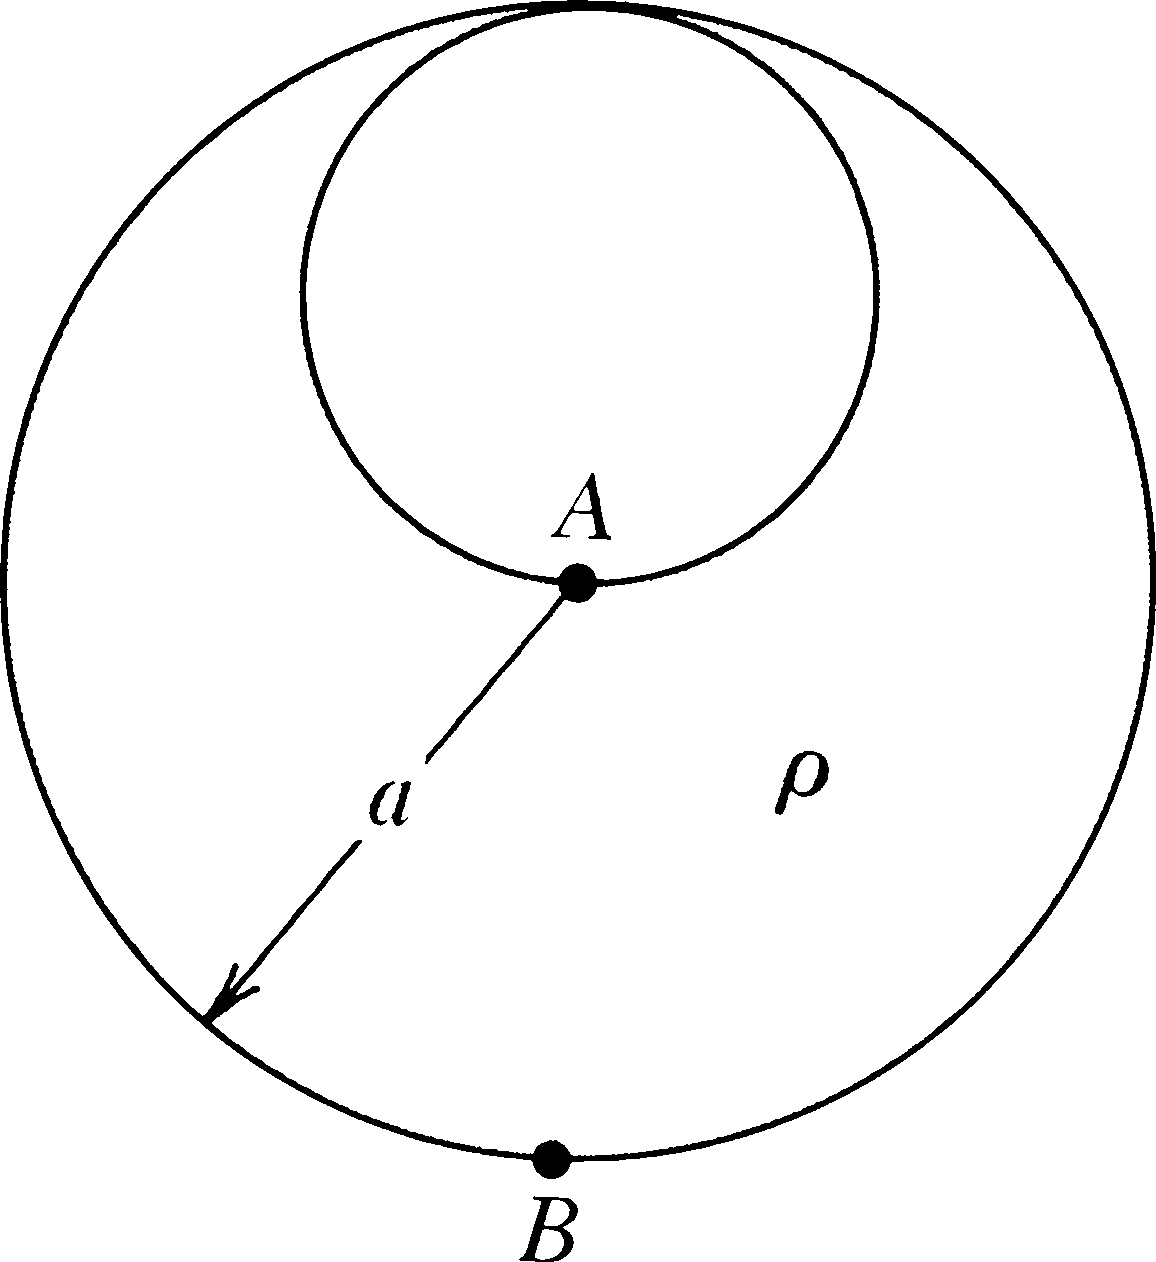
\includegraphics[width=0.3\textwidth]{ps02_1}\end{center}
\subsection{Solution}
  %By the law of superposition, having no charge (density) at a point is the same as having no net charge (density) at that point.  Then the setup is equivalent to calculating the electric field at $A$/$B$ using only the uniform positive charge density, and then superimposing that with the electric field generated by a small negative sphere of uniform density $\rho$ (exactly the same as the sphere carved out).
  %
  %Using the arguments of section 1.11, since both points are not inside the negative sphere, its contribution is the same as if it were a point charge at its center.  By symmetry, the electric field due to the positive sphere, at $A$, is 0.  Then the total electric field at point $A$ is $k\frac{\frac{4}{3}\pi (a/2)^3 \rho}{(a/2)^2} = \frac{2 k \pi\rho}{3}$, pointing towards the center of the smaller sphere.
  %
  %The total electric field at $B$ is $-k\frac{\frac{4}{3}\pi (a/2)^3 \rho}{(3a/2)^2} + k\frac{\frac{4}{3}\pi a^3 \rho}{a^2} = k\frac{4}{3}\pi a\rho\left(1 - \frac{1}{18}\right) = \frac{34}{27}k\pi\rho a$, pointing outwards.
  \begin{figure}[ht]
    \begin{center}
      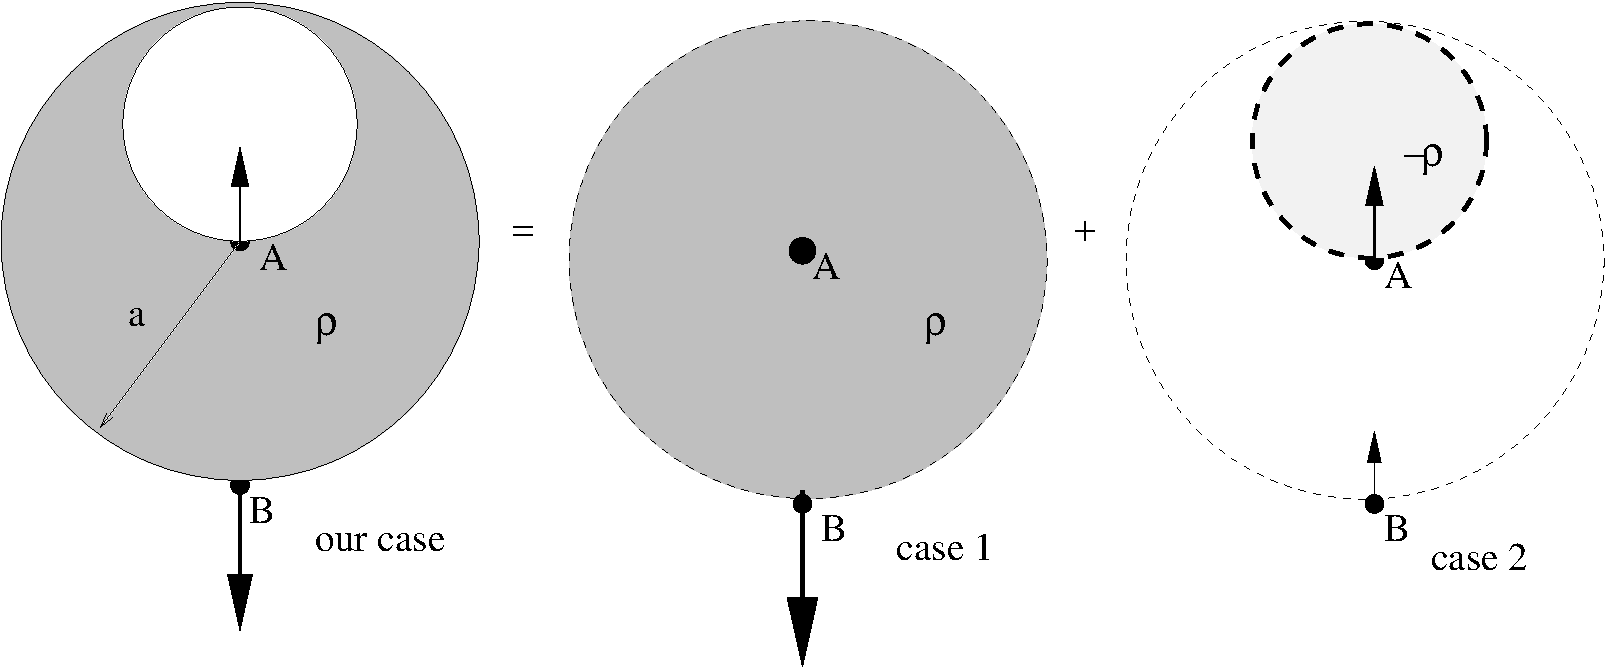
\includegraphics[width=12cm]{ps02_sol_01}
      \caption{A hollow sphere and the equivalent ``decomposition''.}
      \label{fig:hollow5}
    \end{center}
  \end{figure}

  Refer to \autoref{fig:hollow5}.  The hollow sphere (our case) is equivalent to the combination of a solidly charged sphere of uniform density $\rho$ (case 1) and a half-radius sphere of uniform density $-\rho$ (case 2).  Then we can read off the electric field at point A and point B from the figure.
  \begin{align*}
  E_A & = \frac{\rho \frac{4}{3}\pi(a/2)^3}{(a/2)^2} \\
      & = \frac{2}{3}\pi\rho a.
  \end{align*}
  The direction of $\vec E_A$ is upward.
  \begin{align*}
  E_B & = \frac{\rho \frac{4}{3}\pi a^3}{a^2}-\frac{\rho \frac{4}{3}\pi(a/2)^3}{(3a/2)^2} \\
      & = \frac{34}{27}\pi\rho a.
  \end{align*}
  The direction of $\vec{E_B}$ is downward.
\section{Problem \thesection: Purcell 1.17}
\subsection{Problem}
  \begin{enumerate}[(a)]
    \item A point charge $q$ is located at the center of a cube of edge length $d$. What is the value of $\int \vec E \cdot d\vec a$ over one face of the cube?
    \item The charge $q$ is moved to one corner of the cube. What is now the value of the flux of $\vec E$ through each of the faces of the cube?
  \end{enumerate}
\subsection{Solution}
  %\begin{enumerate}[(a)]
    %\item Because the flux of $\vec E$ through any closed surface enclosing a charge $q$ is $4\pi q$.  Since the faces are symmetric, and there are 6 of them, the flux through a face is $\frac{2}{3}\pi q$.
    %\item The electric field is parallel to each of the three faces which meet in that corner, the flux through those faces is zero.  For the other faces, we may imagine them as each a quarter of a face of a cube of edge length $2d$, centered at the new location of the charge.  then the flux through each of these faces is a quarter of the solution to part (a), so the flux is $\frac{1}{6}\pi q$.
  %\end{enumerate}
  \begin{figure}[ht]
    \begin{center}
      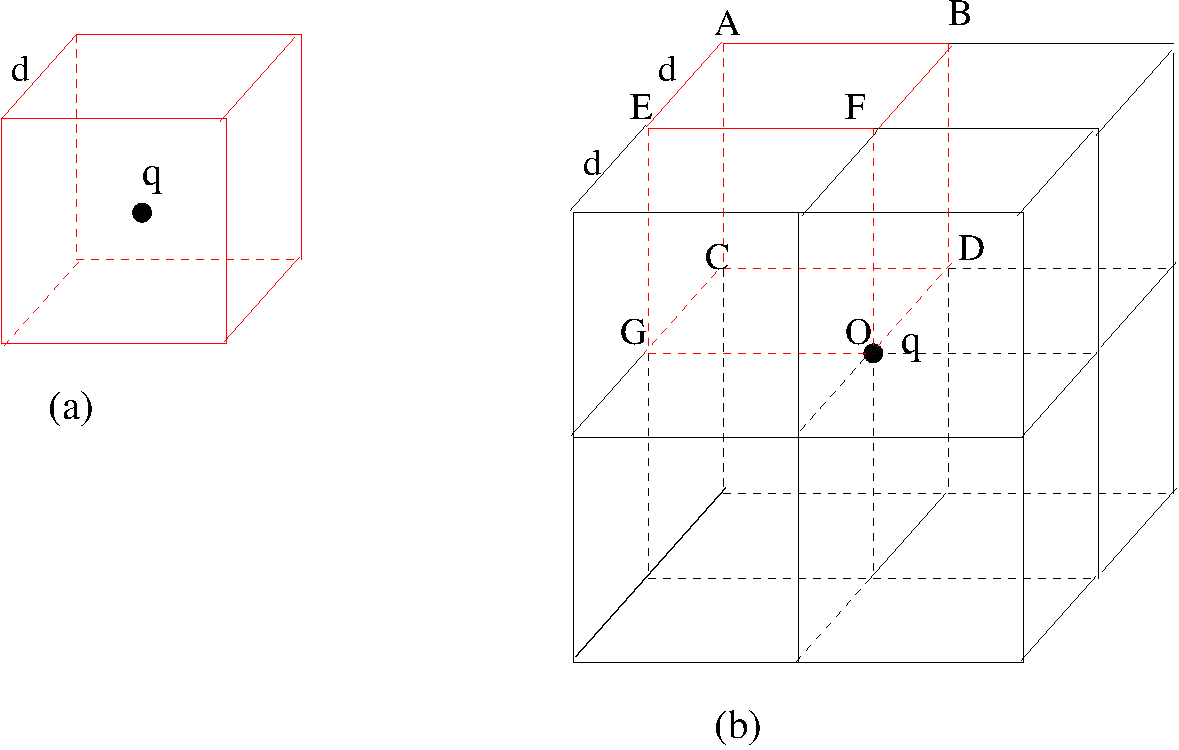
\includegraphics[width=10cm]{ps02_sol_02}
      \caption{A point charge $q$ at the center (a) and at a corner (b) of a cube (the upper-left-back octant of the larger cube; red in color version).}
      \label{fig:cubeflux6}
    \end{center}
  \end{figure}
  \begin{enumerate}[(a)]
    \item Since the point charge $q$ is located at the center of a cube,
          this problem respects the rotational symmetry.  Thus the flux
          $\int\,\vec{E}\cdot d\vec{a}$ is the same for all six faces of the
          cube.  Gauss's law therefore gives
          \begin{align*}
            \int_{one face} \vec{E}\cdot d\vec{a} & = \frac{1}{6}\oint \vec{E}\cdot d\vec{a}\\
                                                  & = \frac{1}{6}\times 4\pi q\\
                                                  & = \frac{2}{3}\pi q.
          \end{align*}
    \item $q$ is now at a corner of the cube.  Imagine we assemble seven
          other identical cubes together as in fig.\ref{fig:cubeflux6}(b).  In
          the new big cube of edge length $2d$, the charge $q$ is again located
          in its center.  Due to the rotational symmetry, we conclude the fluxes
          through three faces ABCD, AEGC, AEFB are the same and each is equal to
          one-quarter of the flux through one face of the big cube.  Therefore
          \begin{align*}
            \int_{ABCD} \vec{E}\cdot d\vec{a}=\int_{AEGC}=\int_{AEFB} & = \frac{1}{4}\times\frac{2}{3}\pi q\\
              & = \frac{1}{6}\pi q.
          \end{align*}
          The fluxes through the other faces, OFEG, OFBD, ODCD are zero since the
          electric field is parallel to these faces, so $\vec{E}\cdot d\vec{a}=0$.
  \end{enumerate}
\section{Problem \thesection: Purcell 1.31}
\subsection{Problem}
  A charged soap bubble experiences an outward electrical force on every bit of its surface. Given the total charge $Q$ on a bubble of radius $R$, what is the magnitude of the resultant force tending to pull any hemispherical half of the bubble away from the other half? (Should this force divided by $2\pi R$ exceed the surface tension of the soap film interesting behavior might be expected!)

  \begin{flushright}\emph{Ans}. $Q^2/8R^2$.\end{flushright}
\subsection{Solution}
  %As determined by pages 30-31, the infinitesimal force is $d\vec F = 2\pi \sigma^2 \hat n dA$ (equation 30).  Then the force for a hemisphere is $\int 2\pi\sigma\hat n dA$.  Transforming the integral to integrate over rings, since the area of a ring is $2\pi (R\cos\theta) (R\Delta \theta)$, \begin{align*}
  %F & = \int_0^{\frac{\pi}{2}}(2\pi\sigma^2)\sin\theta(2\pi\cos\theta R^2) d\theta \\
    %& = \int_0^{\frac{\pi}{2}}(2\pi\sigma^2)\sin2\theta \pi R^2  d\theta \\
    %& = (2\pi^2\sigma^2 R^2)\int_0^{\pi}\frac{1}{2}\sin\theta d\theta \\
    %& = 2\pi^2\sigma^2 R^2 \\
    %\intertext{Since $\sigma = \frac{Q}{4\pi R^2}$, }
  %F & = \frac{2\pi^2 Q^2 R^2}{16 \pi^2 R^4} \\
    %& = \frac{Q^2}{8R^2}
  %\end{align*}

  In class, we derived that the pressure exerted by the electric field
  in a spherical shell is equal to
  $$P = 2\pi \sigma^2 = 2\pi \left(\frac{Q}{4\pi R^2}\right)^2 = \frac{Q^2}{8\pi R^4}.$$

  The area of a small area element is $R^2\sin\theta\,d\theta\,d\phi$.  (See diagram below.)
  \begin{center}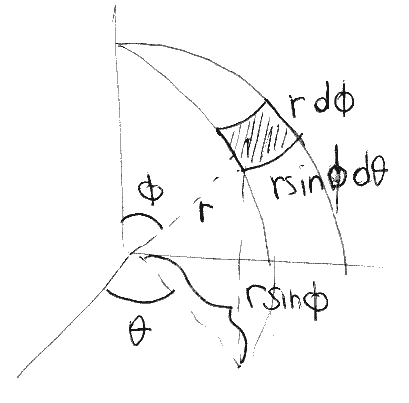
\includegraphics[width=0.35\textwidth]{ps02_sol_03}\end{center}

  For a small area element $dA$, the force is given by
  $$\vec{dF} = P(dA)\hat r = \frac{Q^2}{8\pi R^4}(R^2\sin\theta\,d\theta\,d\phi)\hat r.$$

  Due to the symmetry of the problem, the net force on the hemisphere
  is directed along $\hat z$.

  \begin{align*}
    \vec F & = \sum \delta \vec F_z \\
           & = \sum \delta \vec F \cos\theta\hat z \\
           & = \hat z \int_0^{2\pi}\,d\phi\int_0^{\pi / 2}\sin\theta\cos\theta\,d\theta \frac{Q^2}{8\pi R^2} \\
           & = 2\pi \frac12 \frac{Q^2}{8\pi R^2} \\
           & = \frac{Q^2}{8 R^2}
  \end{align*}



  %\begin{figure}[ht]
    %\begin{center}
      %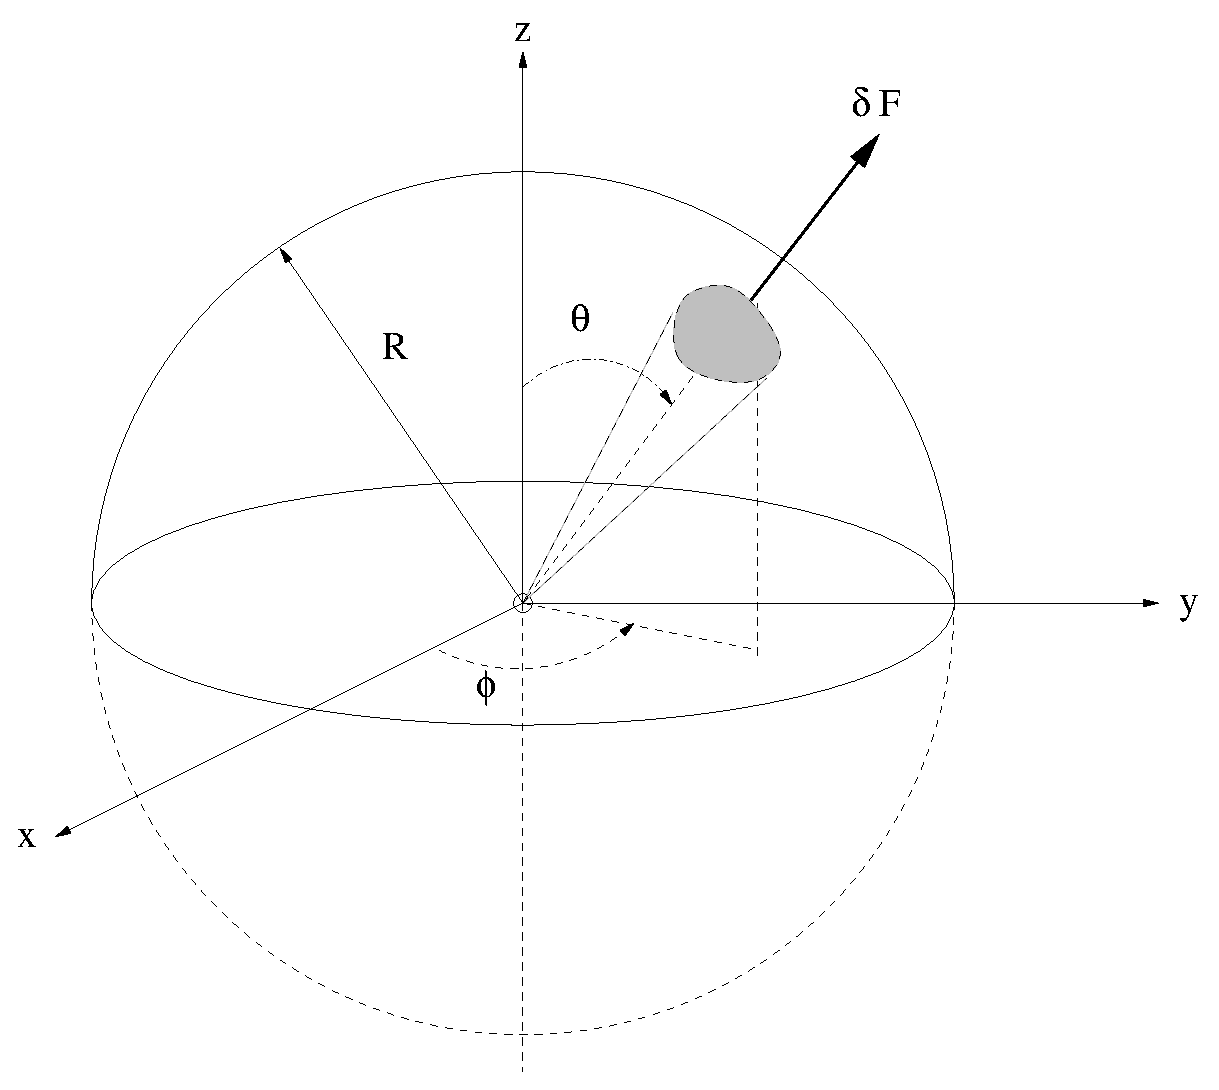
\includegraphics[width=9cm]{ps02_sol_03_old}
      %\label{fig:bubble1}
      %\caption{A spherical bubble on which charges are uniformly distributed.}
    %\end{center}
  %\end{figure}
%
  %Refer to \autoref{fig:bubble1} in which we want to calculate the
  %total force on the upper hemisphere.  For any piece of area element
  %$dA$, the force is pointing outward from the origin; applying eq.(35) of
  %Purcell ch.1,
  %\begin{equation*} F = \frac12 (E_1 + E_2)\sigma \end{equation*}
  %(note that ``F'' in eq.(35) is the force per unit area),
  %the magnitude is determined by
%
  %\begin{align}
    %\delta F & = \frac{1}{2}(E_{inner}+E_{outer})\, \sigma\, dA \nonumber \\
             %& = \frac{Q^2}{8\pi R^2}\sin{\theta}d\theta d\phi, \nonumber \\
    %\text{where,}\qquad\qquad\qquad E_{\text{inner}} & = 0,\nonumber\\
    %E_{\text{outer}} & = 4\pi\sigma,\label{eqn:bubble1}\\
    %dA & = R^2\sin{\theta}d\theta d\phi \nonumber\\
    %\sigma & = Q/(4\pi R^2). \nonumber
  %\end{align}
  %\autoref{eqn:bubble1} is easily seen by eq.(31) of Purcell ch.1,
  %\begin{equation*} E_2 - E_1 = 4 \pi \sigma. \end{equation*}
  %The projected
  %component of $\delta F$ on X-Y plane should be completely canceled throughout
  %the hemisphere as $\sigma$ is constant.  So the net force on the
  %hemisphere is the sum of the z-component of $\delta F$, i.e.
  %\begin{align*}
    %F & = \sum \delta F\cos{\theta} \\
      %& = \int_0^{\pi/2}d\theta\int_0^{2\pi}d\phi\frac{Q^2}{8\pi
    %R^2}\sin{\theta}\cos{\theta}\\
      %& = \frac{Q^2}{8R^2}.
  %\end{align*}
\section{Problem \thesection: Purcell 2.1}
\subsection{Problem}
  The vector function which follows represents a possible electrostatic field:

  \begin{align*}
    E_x & = 6xy &
      E_y & = 3x^2 - 3y^2 &
        E_z & = 0
  \end{align*}

  Calculate the line integral of $\vec E$ from the point $(0, 0, 0)$ to the point $(x_1, y_1, 0)$ along the path which runs straight from $(0, 0, 0)$ to $(x_1, 0, 0)$ and thence to $(x_1, y_1, 0)$. Make a similar calculation for the path which runs along the other two sides of the rectangle, via the point $(0, y_1, 0)$. You ought to get the same answer if the assertion above is true. Now you have the potential function $\phi(x, y, z)$. Take the gradient of this function and see that you get back the components of the given field.
\subsection{Solution}
  \begin{center}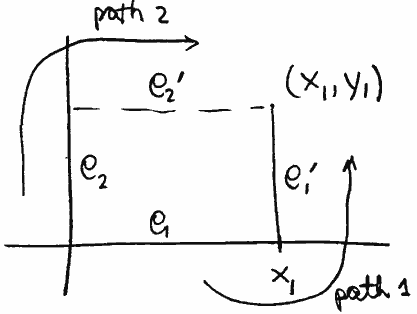
\includegraphics[width=0.25\textwidth]{ps02_sol_04}\end{center}

  Compute first along path 1:
  \begin{align*}
    \phi(x_1, y_1, 0) & = -\int_{\text{path 1}} \vec E \cdot d\vec s \\
      & = -\int_0^{x_1} E_x(x, 0, 0)\,dx - \int_0^{y_1} E_y(x_1, y, 0)\,dy \\
      & = -\int_0^{x_1} 0\,dx - \int_0^{y_1} (3x_1^2 - 3y^2),dy \\
      & = -3x_1^2 y_1 + y_1^3
  \end{align*}
  Compute now along path 2:
  \begin{align*}
    \phi(x_1, y_1, 0) & = -\int_{\text{path 2}} \vec E \cdot d\vec s \\
      & = -\int_0^{y_1} E_y(0, y, 0)\,dy - \int_0^{x_1} E_x(x, y_1, 0)\,dx \\
      & = \int_0^{y_1} 3y^2\,dy - \int_0^{x_1}6xy_1\,dx \\
      & = y_1^3 - 3x_1^2y_1
  \end{align*}
  The two results agree!  Since $E_z = 0$, this gives us, taking the origin as the reference point,
  $$\phi(x, y, z) = y^3 - 3x^2 y.$$
  Checking our answer,
  \begin{align*}
    E_x & = -\frac{\partial \phi}{\partial x} = 6xy \\
    E_y & = -\frac{\partial \phi}{\partial y} = -3y^2 + 3x^2 \\
    E_z & = -\frac{\partial \phi}{\partial z} = 0
  \end{align*}
  %\begin{align*}
  %% \int_{(0,0,0)}^{(x_1,y_1,0)} \vec E \cdot d\vec x & = \int_0^1 (E_x(x(t), y(t), z(t)) \hat i + E_y(x(t), y(t), z(t)) \hat j + E_z(x(t), y(t), z(t)) \hat k) \cdot d\vec s(t) \\
  %% \intertext{where $x(t) = x_1t$, $y(t) = y_1t$, $z(t) = 0$, and $\vec s(t) = x(t)\hat i + y(t)\hat j + z(t)\hat k$.  Then}
  %%  & = \int_0^1 (6x(t)y(t) \hat i + (3(x(t))^2 - 3(y(t))^2) \hat j + 0 \hat k) \cdot d(x(t)\hat i + y(t)\hat j + z(t)\hat k) \\
  %%  & = \int_0^1 (6x(t)y(t) \hat i + (3(x(t))^2 - 3(y(t))^2) \hat j + 0 \hat k) \cdot (x'(t)\hat i + y'(t)\hat j + z'(t)\hat k) dt \\
  %%  & = \int_0^1 (6x(t)y(t)x'(t) + (3(x(t))^2 - 3(y(t))^2)y'(t)) dt \\
  %%  & = \int_0^1 \left(6x_1ty_1t\frac{d(x_1t)}{dt} + (3(x_1t)^2 - 3(y_1t)^2)\frac{d (y_1t)}{d t}\right) dt \\
  %%  & = \int_0^1 \left(6x_1^2y_1t^2 + 3x_1^2y_1t^2 - 3y_1^3t^2\right) dt \\
  %%  & = \left(6x_1^2y_1 + 3x_1^2y_1 - 3y_1^3\right)\int_0^1 t^2 dt \\
  %%  & = \left.\left(6x_1^2y_1 + 3x_1^2y_1 - 3y_1^3\right)\frac{t^3}{3}\right|_0^1 \\
  %%  & = 2x_1^2y_1 + x_1^2y_1 - y_1^3 \\
  %%  & = 3x_1^2y_1 - y_1^3 \\
  %%  \\
    %\int_{(0,0,0)}^{(x_1,0,0)} \vec E \cdot d\vec x & = \int_0^{x_1} E_x dx \\
     %& = \int_0^{x_1} 6xy dx \\
     %& = \int_0^{x_1} 0 dx \\
     %& = 0 \\
    %\\
    %\int_{(x_1,0,0)}^{(x_1,y_1,0)} \vec E \cdot d\vec x & = \int_0^{y_1} E_y dy \\
     %& = \int_0^{y_1} (3x^2 - 3y^2) dy \\
     %& = \int_0^{y_1} (3x_1^2 - 3y^2) dy \\
     %& = 3x_1^2y_1 - 3 \int_0^{y_1} y^2 dy \\
     %& = 3x_1^2y_1 - y_1^3 \\
     %\\
     %\int_{(0,0,0)}^{(x_1,y_1,0)} \vec E \cdot d\vec x & = 0 + 3x_1^2y_1 - y_1^3 \\
     %& = 3x_1^2y_1 - y_1^3 \\
     %\\
     %\\
     %\intertext{Using the other sides of the rectangle,}
    %\int_{(0,0,0)}^{(0,y_1,0)} \vec E \cdot d\vec x & = \int_0^{y_1} E_y dy \\
     %& = \int_0^{y_1} (3x^2 - 3y^2) dy \\
     %& = -3\int_0^{y_1} y^2 dy \\
     %& = -y_1^3 \\
    %\\
    %\int_{(0,y_1,0)}^{(x_1,y_1,0)} \vec E \cdot d\vec x & = \int_0^{x_1} E_x dx \\
     %& = \int_0^{x_1} 6xy dx \\
     %& = \int_0^{x_1} 6xy_1 dx \\
     %& = 6y_1\int_0^{x_1} x dx \\
     %& = 3y_1x_1^2 \\
     %\\
     %\int_{(0,0,0)}^{(x_1,y_1,0)} \vec E \cdot d\vec x & = -y_1^3 + 3x_1^2y_1 \\
     %& = 3x_1^2y_1 - y_1^3
  %\end{align*}
%
  %Since $\phi(x, y, z) = 3x^2y - y^3$, $\vec \nabla \phi = 6xy\hat i + (3x^2 - 3y^2)\hat j$, which is what was expected.
\section{Problem \thesection: Purcell 2.4}
\subsection{Problem}
  Describe the electric field that goes with the following potential:
  \begin{align*}
    \phi & = x^2 + y^2 + z^2 & \text{for }x^2 + y^2 + z^2 < a^2 \\
    \phi & = -a^2 + \frac{2a^3}{(x^2 + y^2 + z^2)^{1/2}} & \text{for }a^2 < x^2 + y^2 + z^2
  \end{align*}
  Discuss what happens at the boundary ($x^2 + y^2 + z^2 = a^2$).
\subsection{Solution}
  %Since $\vec E = -\vec \nabla \phi$, $$\vec E(x, y, z) =
   %\begin{cases}
     %-(2x\hat i + 2y\hat j + 2z\hat k) & \text{for }x^2 + y^2 + z^2 < a^2 \\
     %\frac{2a^3}{(x^2 + y^2 + z^2)^{3/2}}(x\hat i + y\hat j + z\hat k) & \text{for }a^2 < x^2 + y^2 + z^2
   %\end{cases}$$
  %Using polar notation, with $\hat r$ radially outward, and $r^2 = x^2 + y^2 + z^2$,
  %$$\vec E(r) =
   %\begin{cases}
     %-2r\hat r & \text{for }r < a \\
     %\frac{2a^3}{r^2}\hat r & \text{for }a < r
   %\end{cases}$$
%
  %Since $E\cdot A = 4\pi q$, $4\pi \left(\rho\frac43\pi r^3\right) = (-2r)(4\pi r^2) = -8\pi\frac{r^3}{3}$, so $\rho = -\frac{3}{2\pi}$ for $r<a$.
  %Since $E\cdot A = 4\pi q$, $4\pi q = 2a (4\pi a^2)$, so $q_{r\leq a} = 2a^3$.
  %This corresponds to sphere of radius $r$ with charge density $-\frac{3}{2\pi}$, and a shell at radius $a$ of charge $4a^3$.
  For $x^2+y^2+z^2<a^2$, $\phi=x^2+y^2+z^2$,
  \begin{align*}
    \vec{E} & = -\nabla\phi\\
            & = -\frac{\partial\phi}{\partial x}\hat{\bf x}
    -\frac{\partial\phi}{\partial y}\hat{\bf y}
    -\frac{\partial\phi}{\partial z}\hat{\bf z}\\
            & = -2x\hat{\bf x}-2y\hat{\bf y}-2z\hat{\bf z},
  \end{align*}
  or $\vec{E}=(E_x,E_y,E_z)=(-2x,-2y,-2z)$.
  %\begin{align*}
    %\rho & = \frac{1}{4\pi}\nabla\cdot\vec{E}\\
         %& = \frac{1}{4\pi}(\frac{\partial E_x}{\partial x}+
    %\frac{\partial E_y}{\partial y}+\frac{\partial E_z}{\partial z})\\
         %& = -\frac{3}{2\pi}.
  %\end{align*}
  For $x^2+y^2+z^2>a^2$, $\phi=-a^2+\frac{2a^3}{(x^2+y^2+z^2)^{1/2}}$,
  \[\vec{E}=\left(\frac{2a^3 x}{(x^2+y^2+z^2)^{3/2}}\right)\hat{\bf x}+
  \left(\frac{2a^3 y}{(x^2+y^2+z^2)^{3/2}}\right)\hat{\bf y}+
  \left(\frac{2a^3 z}{(x^2+y^2+z^2)^{3/2}}\right)\hat{\bf z}.\]
  %\[\rho=0.\]
  That's not the end of the story: we should be careful of the boundary!
  Take a limit of $x^2+y^2+z^2\rightarrow a^2$ from both inside and
  outside; the fields are not the same.  This indicates there are some surface
  charge density $\sigma$ on the boundary $x^2+y^2+z^2=a^2$.  Let
  $a^-\equiv \lim_{\varepsilon\rightarrow 0,\varepsilon>0}(a-\varepsilon)$
  and $a^+\equiv \lim_{\varepsilon\rightarrow
  0,\varepsilon>0}(a+\varepsilon)$.
  \begin{align*}
    \vec{E_1}& = \vec{E}\left(x^2+y^2+z^2=(a^-)^2\right)=-2x\hat{\bf x}-2y\hat{\bf y}-2z\hat{\bf
      z}\\
    \vec{E_2}& = \vec{E}\left(x^2+y^2+z^2=(a^+)^2\right)= 2x\hat{\bf x}+2y\hat{\bf y}+2z\hat{\bf
      z}\\
    |\vec{E_2}-\vec{E_1}|& = |4x\hat{\bf x}+4y\hat{\bf y}+4z\hat{\bf z}|\\
      & = 4\sqrt{x^2+y^2+z^2}=4a\\
    \sigma & = |\vec{E_2}-\vec{E_1}|/4\pi =+a/\pi.
  \end{align*}
\section{Problem \thesection: Purcell 2.8}
\subsection{Problem}
  For the cylinder of uniform charge density in Fig. 2.17:
  \begin{enumerate}[(a)]
    \item Show that the expression there given for the field inside the cylinder follows from Gauss's law.
    \item Find the potential $\phi$ as a function of $r$, both inside and outside the cylinder, taking $\phi = 0$ at $r = 0$.
  \end{enumerate}
  \begin{center}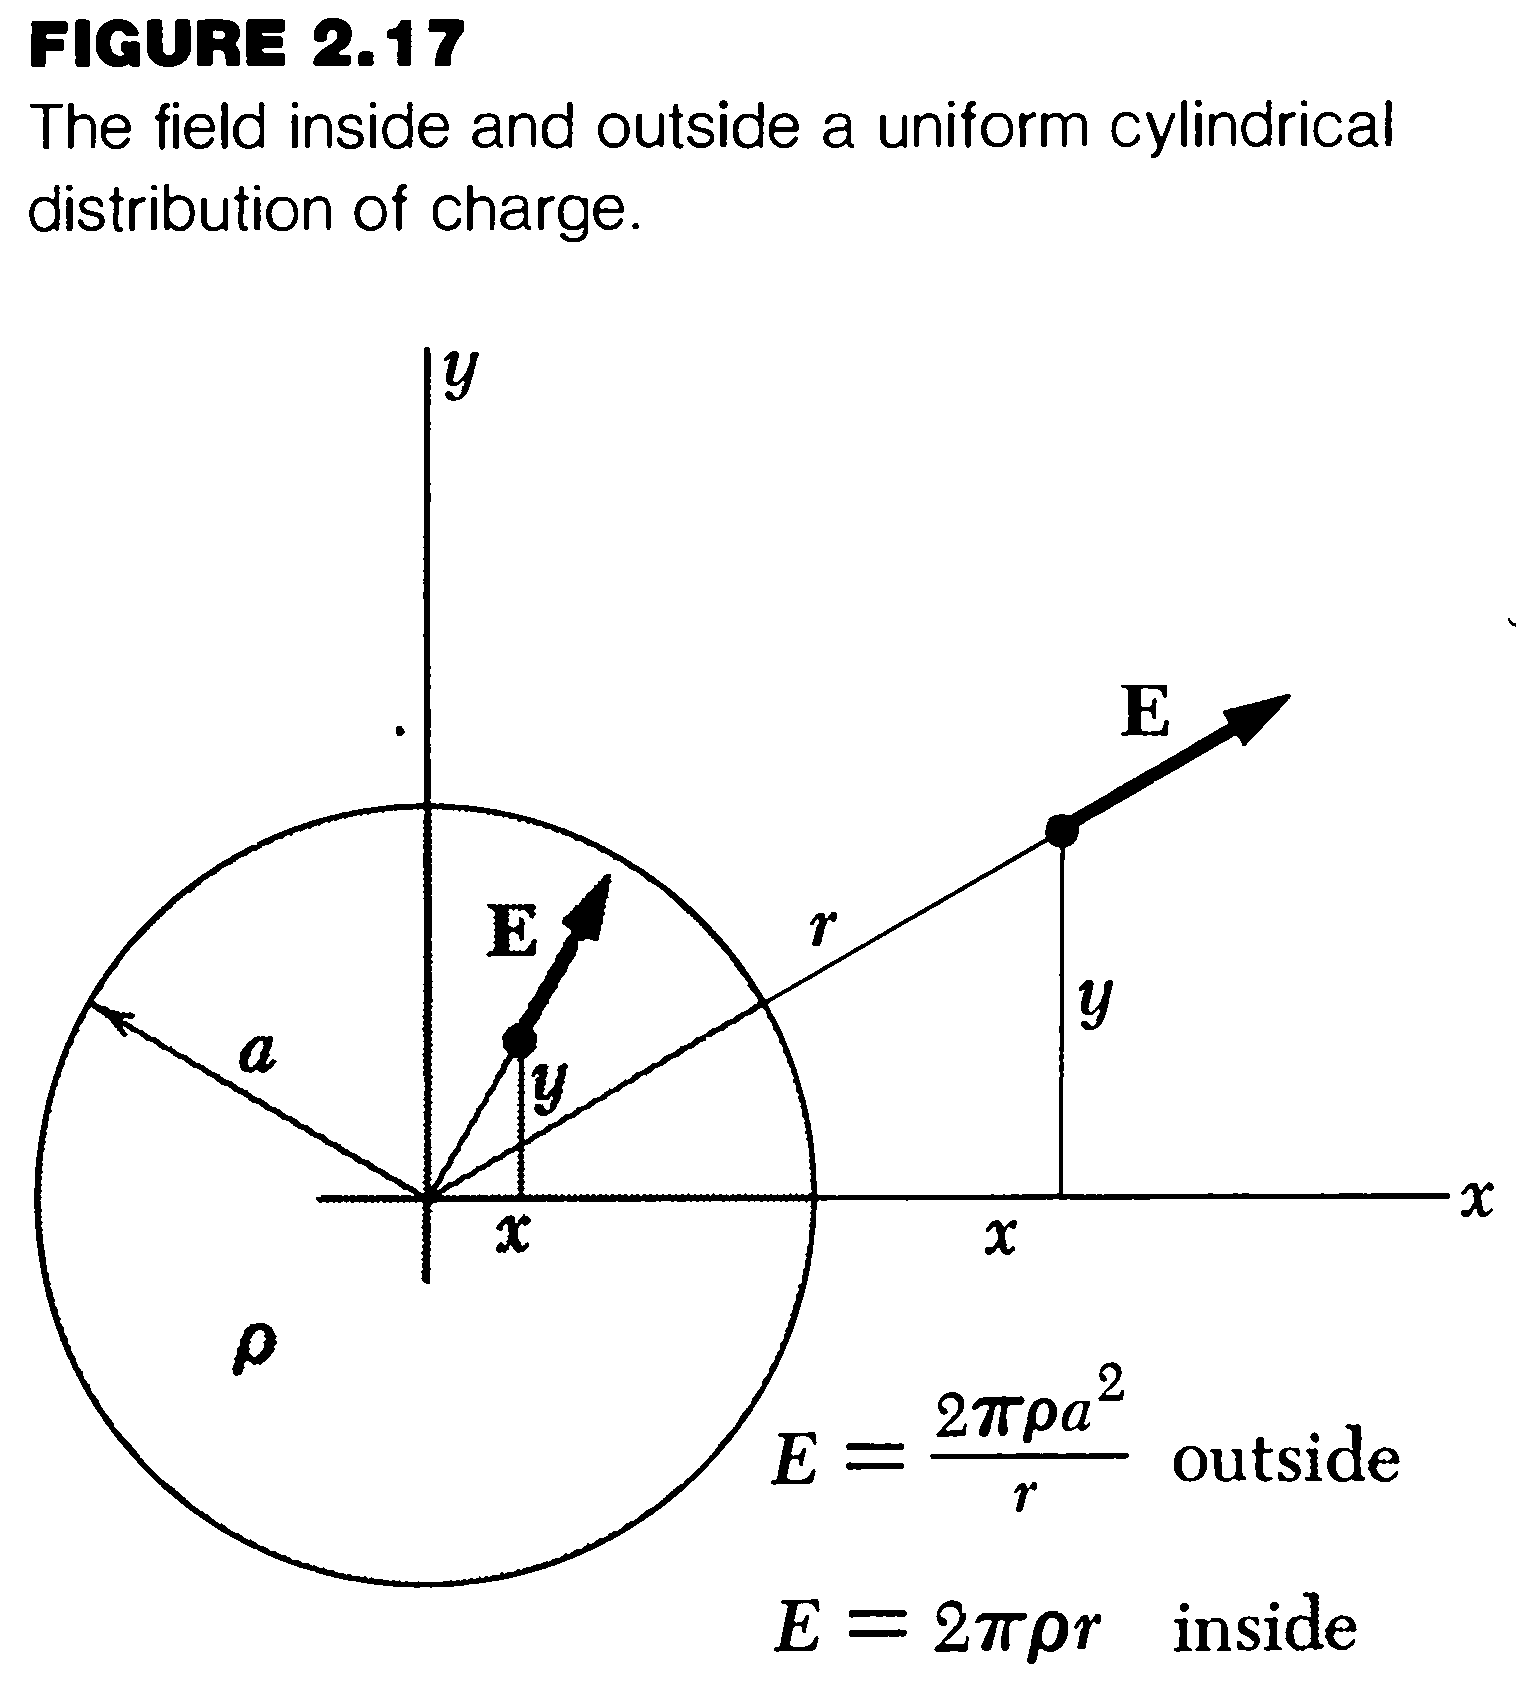
\includegraphics[width=0.4\textwidth]{ps02_2}\end{center}
\subsection{Solution}
  %\begin{enumerate}[(a)]
    %\item By symmetry, the field must be radial.  Applying, in two dimensions, the argument that shows that the electric field at a point inside a uniformly charged sphere is due only to the charge further inside the sphere than that point, we get that the electric field at radius $r$ in the cylinder is due entirely to the charge at a radius less than or equal to $r$.  Apply Gauss' law to a segment of the cylinder, of length $\ell$ and radius $r$, which has volume $\ell \pi r^2$.  By symmetry, and since the electric field must be radial in direction, it is zero through the ends of the cylinder-segment, and uniform through the cylindrical surface.  Then, since the surface area is $\ell 2\pi r$,  $\ell 2\pi r E(r) = A \cdot E(r) = 4\pi q_{\text{enc}} = 4\pi (\rho \ell \pi r^2)$, so $E(r) = 2\pi \rho r$.
    %\item Since $\phi(0) = 0$, $\phi(r) = -\int_0^r \vec E \cdot d\vec r'$.  Since both $\vec r'$ and $\vec E$ point outward for a positive charge density, $\phi(r) = -\int_0^r 2\pi \rho r'\, dr' = -2\pi\rho \frac{1}{2}r^2 = -\pi\rho r^2$ for $r < a$.  For $r > a$, $\phi(r) = -\pi\rho r^2 - \int_a^r \frac{2\pi \rho a^2}{r'}\, dr' = -\pi\rho\left(r^2 + 2a^2\int_a^r \frac{1}{r'}\, dr'\right) = -\pi\rho\left(r^2 + 2a^2(\ln r - \ln a)\right) = -\pi\rho\left(r^2 + 2a^2\ln \frac{r}{a}\right)$.  This is $$\phi(r) = \begin{cases} -\pi\rho r^2 & r < a \\ -\pi\rho\left(r^2 + 2a^2\ln \frac{r}{a}\right) & r > a \end{cases}$$
  %\end{enumerate}
  \begin{figure}[ht]
    \begin{center}
      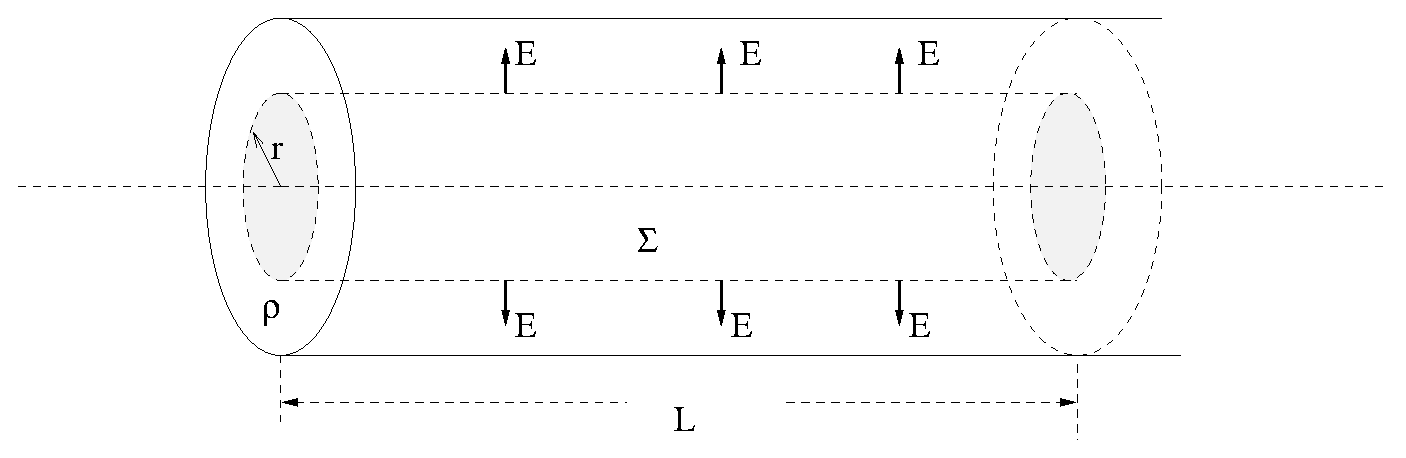
\includegraphics[width=12cm]{ps02_sol_05}
      \caption{A cylinder inside which charges are uniformly
      distributed. The fields are along radial direction.}
      \label{fig:cylinder3}
    \end{center}
  \end{figure}

  \begin{enumerate}[(a)]
    \item The symmetry of a cylinder contains the direction of the field
      $\vec{E}$ to be radial.  Refer to figure \ref{fig:cylinder3}.  We
      consider a cylindrical closed surface $\Sigma$ whose radius is $r$ and
      length is $L$.  The flux on the two cross sections are zero.  So
      \begin{align*}
        \oint \vec{E}\cdot d\vec{A} & = 4\pi Q_{\text{inside}}\\
        E\times(2\pi rL) & = 4\pi\rho\pi r^2L
      \end{align*}
      or
      \begin{equation*}
      E=2\pi\rho r,
      \end{equation*}
      for $r<a$.  Similarly, we can work out the field outside the cylinder
      by Gauss's law,
      \begin{equation*}
      E=2\pi\rho a^2/r,
      \end{equation*}
      for $r>a$.
    \item For $r<a$,
      \begin{align*}
        \phi(r) & = -\int_0^r\vec{E}\cdot d\vec{r}+\phi(0)\\
                & = -\int_0^r 2\pi\rho r\,dr+0\\
                & = -\pi\rho r^2.
      \end{align*}
      For $r>a$,
      \begin{align*}
        \phi(r) & = -\int_a^r \vec{E}\cdot d\vec{r}+\phi(a)\\
                & = -\int_a^r\frac{2\pi\rho a^2}{r}dr-\pi\rho a^2\\
                & = -2\pi\rho a^2\ln{(r/a)}-\pi\rho a^2.
      \end{align*}
  \end{enumerate}
\section{Problem \thesection: Purcell 2.12}
\subsection{Problem}
  The right triangle with vertex $P$ at the origin, base $b$, and altitude $a$ has a uniform density of surface charge $\sigma$. Determine the potential at the vertex $P$. First find the contribution of the vertical strip of width $dx$ at $x$. Show that the potential at $P$ can be written as $\phi_P = \sigma b \ln[(1 + \sin \theta) / \cos \theta]$.
  \begin{center}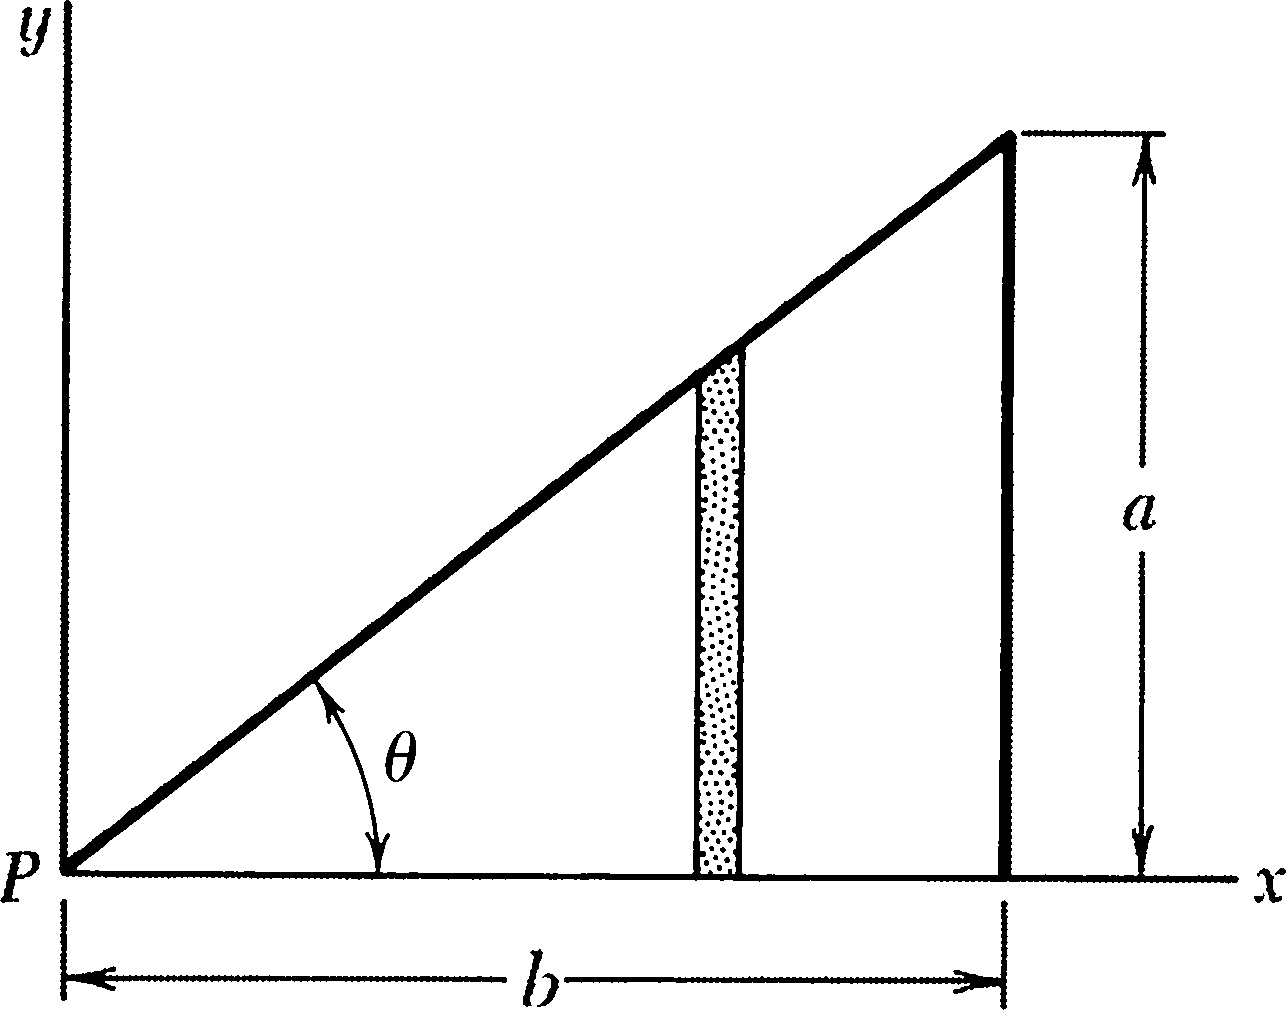
\includegraphics[width=0.35\textwidth]{ps02_3}\end{center}
\subsection{Solution}
  %The contribution of the vertical strip is $\int_0^{x \tan\theta} \frac{\sigma\,dx\, dy}{\sqrt{x^2 + y^2}}$.  Substituting $y = x\tan\theta'$, $dy = x\sec^2\theta'\, d\theta'$, so the contribution of the vertical strip is $\sigma\,dx \int_0^{\theta} \frac{x\sec^2\theta'\, d\theta'}{\sqrt{x^2 + x^2\tan^2\theta'}} = \sigma\,dx \int_0^{\theta} \frac{\sec^2\theta'\, d\theta'}{\sec\theta'} = \sigma\,dx \int_0^{\theta} \sec\theta'\, d\theta'$.  Since $\frac{d}{d\theta}\ln\frac{1+\sin\theta}{\cos\theta} = \sec\theta$, the contribution of the vertical strip is $\sigma\,dx\ln\frac{1+\sin\theta}{\cos\theta}$.  Then the potential at $P$ can be written as $\phi_P = \sigma \ln\frac{1+\sin\theta}{\cos\theta} \int_0^b dx = \sigma b\ln\frac{1+\sin\theta}{\cos\theta}$.
  \begin{center}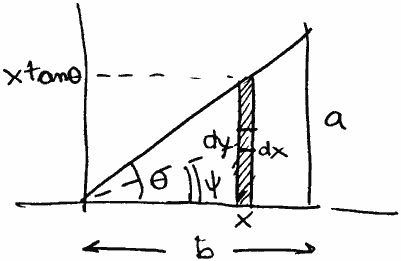
\includegraphics[width=0.35\textwidth]{ps02_sol_06}\end{center}
  To get the potential due to the little vertical strip:
  \begin{align*}
    d\phi_{\text{strip}} & = \frac{\sigma\,dA}{r} \\
    \intertext{where $dA = dx\,dy$}
    \phi_{\text{strip}} & = \smashoperator{\int}_{y=0}^{y=x\tan\theta} \frac{(\sigma\,dx)\,dy}{\sqrt{x^2+y^2}} \\
      & = \sigma\,dx\smashoperator{\int}_{y=0}^{y=x\tan\theta} \frac{dy}{\sqrt{x^2+y^2}}
  \end{align*}
  It is actually good to change variables to $\psi$:

  Let $y = x\tan\psi$ so that $dy = \frac{x}{\cos^2\psi}\,d\psi$.  Then
  \begin{align*}
    \phi_{\text{strip}} & = \sigma\,dx\int_{0}^\theta \left(\frac{x\,d\psi}{\cos^2\psi}\right)\frac{1}{x\sqrt{1 + \tan^2\psi}} \\
    \intertext{Since $1 + \tan^2\psi = \sec^2\psi = 1 / \cos^2\psi$,}
      & = \sigma\,dx\int_{0}^\theta \frac{d\psi}{\cos\psi} \\
      & = \sigma\,dx\ln|\sec\theta + \tan\theta| \\
      & = \sigma\,dx\ln\left|\frac{1 + \sin\theta}{\cos\theta}\right| \\
  \end{align*}
  Now:
  \begin{align*}
    \phi_{\text{tot}} & = \int_{x=0}^{x=b}\phi_{\text{strip}} \\
      & = \int_0^b \sigma\,dx\ln\left|\frac{1 + \sin\theta}{\cos\theta}\right| \\
      & = \sigma b \ln\left|\frac{1 + \sin\theta}{\cos\theta}\right|
  \end{align*}
  Check: As $\theta \to 0$, $\phi_{\text{tot}} \to \sigma b \ln 1 = 0$.
\section{Problem \thesection: Purcell 2.30}
\subsection{Problem}
  Consider a charge distribution which has the constant density $\rho$ everywhere inside a cube of edge $b$ and is zero everywhere outside that cube. Letting the electric potential $\phi$ be zero at infinite distance from the cube of charge, denote by $\phi_0$ the potential at the center of the cube and $\phi_1$ the potential at a corner of the cube. Determine the ratio $\phi_0/\phi_1$. The answer can be found with very little calculation by combining a dimensional argument with superposition. (Think about the potential at the center of a cube with the same charge density and with twice the edge length.)
\subsection{Solution}
  %Let $\phi_1$ denote the potential at the corner of a cube with edge $b$, and $\phi_0$ denote the potential at the center of a cube of edge $b$.  Because we may superimpose the scalar fields $\phi$ for different cubes, electric potential at the center of a cube of edge $2b$ is $8\phi_1$.  Since $\phi = \int E\cdot \d s \propto \frac{q}{r} \propto \frac{\rho r^3}{r} \propto r^2$, $\phi\propto b^2$.  Then the potential at the center of a cube of edge $2b$ is $4\phi_0$.  Then $\phi_0 / \phi_1 = 2$.
%
  Let's do dimensional analysis.  The potential $\phi_0$ at the center
  is proportional to the total charge of the cube and inversely
  proportional to the characteristic length $b$, i.e.
  \begin{equation*}
    \phi_0 = c \frac{\rho b^3}{b}= c \rho b^2 \propto b^2,
  \end{equation*}
  where $c$ is a constant depending only on the shape of the object.  If
  we assemble eight identical cubes together, each of which has the same
  charge density $\rho$ and edge length $b$, the potential $\phi'_0$ at
  the \emph{new} center is four times the previous $\phi_0$.  Note that the center of the
  \emph{bigger} cube is a corner of the previous small cube; so
  $\phi'_0=8\phi_1$.  There we get $4\phi_0=\phi'_0=8\phi_1$, or
  \[\frac{\phi_0}{\phi_1}=2.\]

  Graphically, treating $\phi_0$ as a function of charge distribution, this is
  \begin{center}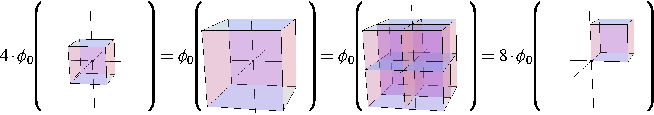
\includegraphics[width=\textwidth]{ps02_sol_07}\end{center}
  %%%%%%%%%%%%%%%%%%%%%%%%%%%%%%%%%%%%%%%%%%%%%%%%%%%%%%%%%%%%%%%%%%% Mathematica Code for diagram %%%%%%%%%%%%%%%%%%%%%%%%%%%%%%%%%%%%%%%%%%%%%%%%%%%%%%%%%%%%%%%%%%%
  %Clear[LineAxes, GraphicsVars, GraphicsOpts, ShowOpts, CubeSmall, \
%CubeLarge, Cube8, CubePart, expr, \[Phi]]
%LineAxes[min_, max_] :=
 %Map[Line[{min, max} {#, #}] &, {{1, 0, 0}, {0, 1, 0}, {0, 0, 1}}]
%GraphicsVars =
  %Sequence[LineAxes[-1.5, 1.5], PointSize[0.02], Point[{0, 0, 0}],
   %Opacity[0.25]];
%GraphicsOpts = Boxed -> False;
%ShowOpts =
  %Sequence[ImageSize -> Medium, ViewPoint -> {-\[Pi], -0.8, -0.9},
   %ViewVertical -> {-0.35, -0.9, -0.136}];
%CubeSmall =
  %ImageCrop[
   %Show[Graphics3D[{GraphicsVars,
      %Cuboid[{-1, -1, -1}/2, {1, 1, 1}/2]}, GraphicsOpts], ShowOpts]];
%CubeLarge =
  %ImageCrop[
   %Show[Graphics3D[{GraphicsVars, Cuboid[{-1, -1, -1}, {1, 1, 1}]},
     %GraphicsOpts], ShowOpts]];
%Cube8 = ImageCrop[
   %Show[Graphics3D[{GraphicsVars,
      %Table[Cuboid[{0, 0, 0}, {(-1)^i, (-1)^j, (-1)^k}], {i, 0,
        %1}, {j, 0, 1}, {k, 0, 1}]}, GraphicsOpts], ShowOpts]];
%CubePart =
  %ImageCrop[
   %Show[Graphics3D[{GraphicsVars, Cuboid[{0, 0, 0}, {1, -1, -1}]},
     %GraphicsOpts], ShowOpts]];
%expr = TraditionalForm[
  %4\[CenterDot]Defer[Subscript[\[Phi], 0]][CubeSmall] ==
   %Defer[Subscript[\[Phi], 0]][CubeLarge] ==
   %Defer[Subscript[\[Phi], 0]][Cube8] ==
   %8\[CenterDot]Defer[Subscript[\[Phi], 0]][CubePart]]
%Export["ps02_sol_8__2_30_1.pdf", expr]
  %%%%%%%%%%%%%%%%%%%%%%%%%%%%%%%%%%%%%%%%%%%%%%%%%%%%%%%%%%%%%%%%%%%%%%%%%%%%%%%%%%%%%%%%%%%%%%%%%%%%%%%%%%%%%%%%%%%%%%%%%%%%%%%%%%%%%%%%%%%%%%
\end{document}
